 \section{Introduction}

  Having a fast and reliable internet connection is something that individuals and compagnies would want.

  Nowadays, there are multiple solutions to this, for example compagnies can get a fiber optic connection but it is still very expensive.

  Individual or small entreprise have Multihoming. It uses multiple internet connections at the same time and balances traffic amongst them using a router configured especially for that.
  Unfortunatly it does not always improve the speed of the connection and can be slow to react to failures.

  In this paper, I describe and analyse another solution which is less expensive than optic fiber and will make better use of brandwidth
  and be more tolerant to failures than Multihoming. This solution implies using MultiPath TCP, OpenVPN and OpenWRT.

  Multipath TCP (MPTCP) has been implemented by the IP Networking Lab at Université catholique de Louvain(UCL) in Louvain-la-Neuve for the linux kernel. It is an extension of the TCP protocol,
  and it's goal is to support the use of multiple transport paths between a pair of hosts.
  The benefits of MPTCP include a performance improvement in term of throughput and a better handling of failures.

  OpenVPN is an open source application implementing a virtual private network (VPN) to create secure connections between hosts over a network.
  OpenWrt is a linux distribution for embedded devices typically home routers. It is built from the ground up to be a full-featured, easily modifiable and light weight operating system.

  In this setup, MPTCP will be use to balance the traffic between multiple internet connections and recover from a possible failure of one of them.
  OpenVPN will be use to create the link between the MPTCP compatible server and the home router running a modified version of OpenWRT supporting MPTCP.
  For this to work, the user/entreprise should have two or more internet connections and a server with a high brandwith running a MPTCP kernel.

  The goal of the solution described in this paper is to give the possibility to more people to get a fast and reliable internet connection.

  This paper will first present the theory about multipath TCP and Virtual Private Network in Chapter 1. Chapter 2 describes the setup of the experiment and the tests operated.
  The results of these tests are presented in Chapter 3. Chapter 4 is an attempt to develop solutions to the problems encountered duriing the test. Finally, Chapter 5 presents the tools used
  to perform the tests and Chapter 6 concludes the report.

  \section{Multipath TCP (MPTCP)} \label{sec:mptcp_exp}

  Multipath TCP has been implemented by the IP Networking Lab at Université catholique de Louvain(UCL) in Louvain-la-Neuve for the linux kernel.
  MPTCP is an attempt to solve problems of the TCP protocol : the inability to move TCP connection from one IP to another and the inability to use more than one path for a single TCP connection.
  Many attempts have been made but some involve changes in the applications and others lose advantages of current TCP protocol.

  Multipath TCP also need to be backward compatible with normal TCP to ensure that even if the other end is not compatible they can still communicate.
  Another thing to achieve is the fairness between MPTCP and TCP: if MPTCP and normal TCP share a bottleneck link, MPTCP should not be able to use more bandwith than a normal TCP connection.

  \subsection{Architecture}

  Multipath TCP is an extention of the TCP protocol,. It does not change the interface of the socket API for applications which allows all applications to benefit from it
  without need for modification.
  It removes the strong link between IP and TCP so that devices can use multiple IP for a single MPTCP connection.

  MPTC uses TCP options to annonce MPTCP support and communicate MPTCP informations between host.

  The setup of a MPTCP connection is as follow:

  \begin{enumerate}
    \item First the initiator of the connection annonces that he is MPTCP compatible (MP\_CAPABLE)
    \item Then if the receiver is MPTCP compatible, it establish a new MPTCP connection
    \item After that, it adds new subflow on every know path to the existing MPTCP connection (MP\_JOIN)
    \item Finally it transmit data on the MPTCP connection
  \end{enumerate}

  \begin{figure}[h!]
    \centering
    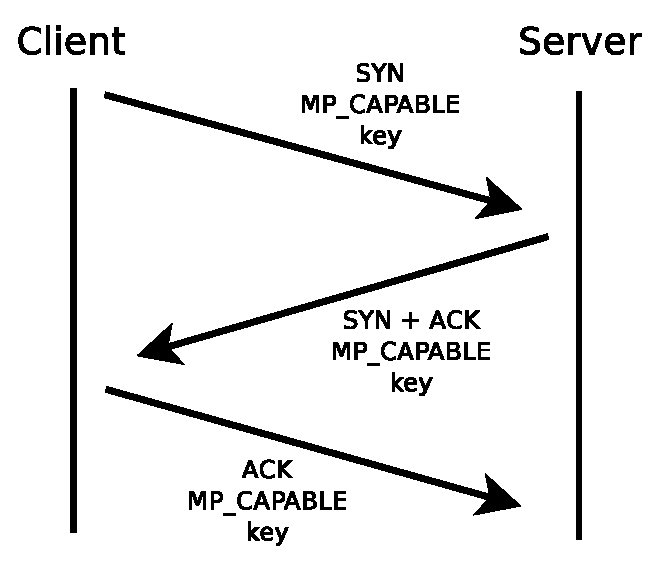
\includegraphics[width=8cm]{./images/mptcp_connection_setup.eps}
    \caption{MPTCP connection setup}
    \label{mptcp_connection_setup}
  \end{figure}


  To establish a MPTCP connection it uses a three-way handshake as show in figure \ref{mptcp_connection_setup}.
  A client send a packet having the MP\_CAPABLE option to tell the server he is compatible.
  The server send back a ACK containing a MP\_CAPABLE option and a random key if it is compatible.
  After that the client send a ACK to the server containing the key, this will setup the first subflow.

  \begin{figure}[h!]
    \centering
    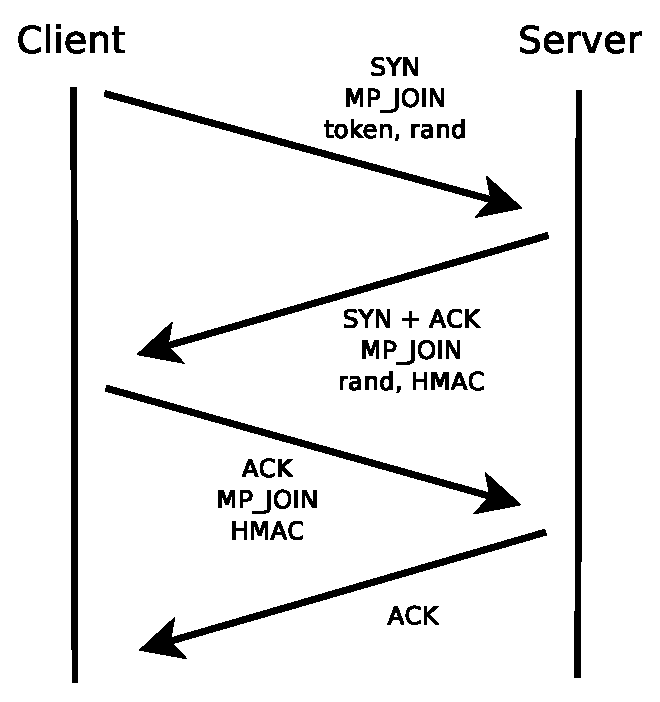
\includegraphics[width=8cm]{./images/mptcp_mp_join.eps}
    \caption{MPTCP Add subflow}
    \label{mptcp_mp_join}
  \end{figure}

  If the client has more than one physical link connected with the server, MPTCP will try to add another subflow to the existing connection.
  For this it will use a three-way handshake and the MP\_JOIN option with a unique token.(figure \ref{mptcp_mp_join})

  \begin{enumerate}
    \item First a SYN with the MP\_JOIN Option, a unique token and random key will be sent
    \item Then the client and the server will compute an hash-based message authentification code computed over the random key exchanged.
  \end{enumerate}

  The token is there to be able to uniquely identify a subflow, because in normal TCP a connection is identified by <srcip,srcport,dstip,dstport>
  which in this case is not sufficient to uniquely identify a subflow in case of a host behind a NAT.

  When multiple subflows have been established, data can be transmited over any of them. This can be used to increase the throughput of the connection or
  to retransmit data if one subflow fail. Each subflow is equivalent to a single TCP connection.

  If multiple subflows are use for a single TCP connection MPTCP must decide on which one to send the data and how much data.
  For this purpose, MPTCP use a scheduler, there are two type of scheduler in MPTCP :

  \begin {enumerate}
    \item The default scheduler used by MPTCP will first send data on subflows with the lowest RTT until their congestion-window is full then it will start transmitting on the subflows with the next higher RTT.
    \item The roundrobin scheduler will transmit X consecutive segment on each path in a round robin fashion (X can be changed and default is 1).
  \end{enumerate}

  Using multiple subflows also require to order the data within each subflow and then order the data between these different subflows, because some can be faster than others.
  When receiving data it first reorders them at the subflow level using the subflow sequence number, a 32bits number. Then it reorders the data between the different sublows at the connection level using the data sequence number.

  \subsection{Congestion}

  Congestion control in MPTCP is more complex than with regular TCP because it uses multiples subflows for one connection.
  On these subflows the level of congestion can be very different, if one uses standard TCP congestion algorithm the performance for MPTCP it usually become unfair to regular TCP and
  in some situations decreases the performances.

  To solve that problem a few congestion control algorithms have been developped for MPTCP like LIA, OLIA, wVegas. These algorithms are described below.

  \subsubsection{ Linked Increase Algorithm (LIA)} \label{sec:lia}

  The LIA algorithm has three main goals :

  \begin{enumerate}
    \item Having a total throughput bigger than the one TCP can get using the best path
    \item Not being more aggressive than TCP, be fair to TCP.
    \item Balancing the congestion over paths
  \end{enumerate}

  As it accomplishes the two first goal but fails to accomplish the third one,  a new algorithm has been developped, OLIA.

  In LIA, the slow start, fast retransmit, and fast recovery algorithms, as well as the multiplicative decrease of the congestion avoidance state are the same as in standard TCP.

  What changes is the increase phase of the congestion avoidance state, the window is increased by the minimum between the increase that would get normal TCP and the computed increase
  for the multipath subflow. The computed increase is calculated using a parameter $\alpha$ which defines the aggresiveness of the MPTCP flow. The value of this parameter $\alpha$ is chosen such that the aggregate
  throughput of the multipath flow is equal to the rate a TCP flow would get if it ran on the best path.
  $\alpha$ need to be calculated for each MPTCP flow. The formula which is used has been derived by equalizing the rate of the multipath flow with the rate of a TCP running on the best path.

  This guarantees the goal number two: not being more aggressive than TCP. Goal one is accomplished by computing an increase for the multipath subflow equal to
  the throughput a TCP flow would get if it ran on the best path.

  \subsubsection{ Opportunistic Linked-Increases Algorithm (OLIA)} \label{sec:olia}

  OLIA is a window-based congestion-control algorithm that couples the increase of congestion windows and uses unmodifed TCP behavior in the case of a loss.
  Like LIA, the algorithm only modifies to the increase part of the congestion avoidance phase.

  It uses a set of best paths devided in two, a set with max windows and the rest of the paths. For the paths that have a small windows, OLIA increase the window faster.
  For the path that have the max windows, the increase is slower.

  \subsubsection{ wVegas } \label{sec:wvegas}

  wVegas is a delay-based congestion control based on TCP vegas. It is more sensitive to change because it does not have to wait for packet losses to react and shift between subflows to adapt to network congestion.
  For each subflow it calculate the difference between the expected sending rate and actual sending rate

  During slow-start it double the congestion window every other RTT. If the difference is bigger than a threshold, it switches to congestion-avoidance.
  During congestion-avoidance it increase the window by one packet every RTT if the difference is small otherwise it reduces it by one packet.

  This means that overall the window grow slower than other algorithm and this avoids losses. However when the BDP is large, it switches too fast to the congestion avoiding phase and gives
  bad throughput because the windows is too small.

  \subsection{Usages}

  MPTCP can be use in different fields. It is usefull for devices like smartphones that have multiple network interfaces with different throughput and latency. Today these devices only use one interface at a time and
  if it loses the connection to that interface, all the currently open TCP connection will be terminated and will need to be reopenned.

  This is a situation that MPTCP can solve by having one subflow for the 3G interface and one subflow over the wifi interface: when one subflow fails, the data are sent over the other subflow.

  MPTCP can also be very usefull in data center where different topologies use multiple paths accross the server layer and the traffic need to be balanced between the paths to avoid congestion.

  \section{VPN}

  A Virtual private network provide a point-to-point connection between two or more nodes on top of an existing network, it create a tunnel between the connected nodes.(figure \ref{vpn1})

  In VPN privacy is a concern: The data which are transmited using these virtual network need to be encrypted so that if someone intercept it on the global network, it cannot be read.
  The data are encrypted before entering the tunnel and will be decrypted after leaving it, the VPN will usually add extra header information to the packets for the remote node to be able to decrypt.

  Another technique used in VPN is the authentification. Client and server must provide information about who they are so that they can prove their idendity.
  This is mostly done by using a Message Authentication Code (MAC).

  One of the main motivation for VPN is that it is cheaper to use multiple virtual networks implemented on a global network than use multiple smaller physical networks.
  It is usually used by compagnies to create a private network over the internet.

  There are several types of VPN technologies : Point-to-Point Tunneling Protocol,Secure Socket Layer/Transport Layer Security (SSL/TLS) or Internet Protocol Security.
  They all use the same basic principle to transfert data accross by tunneling it.

  \begin{figure}[h!]
    \centering
    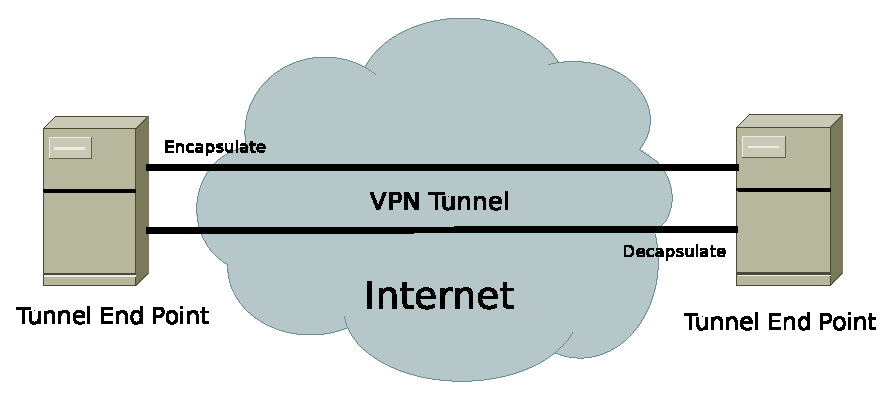
\includegraphics[width=1\textwidth]{./images/vpn1.eps}
    \caption{VPN Tunnel}
    \label{vpn1}
  \end{figure}

  The principle is that the packet is encrypted and encapsulated within another packet which will be delivered to the other node. The node will then decapsulate the packet and decrypt it.

  \subsection{Why using a VPN}

  For this article, we will use a end-to-end, one-to-one connection to connect the router and the server with each other and encapsulate all the clients traffic into the OpenVPN tunnel.

  So even in the case clients do not support MPTCP, all the packets sent by the client will be encapsulated on the router within OpenVPN packet
  and because the router is MPTPC capable, the OpenVPN packets will use MPTCP to transit between the router and the server.

  \subsection{OpenVPN} \label{sec:section_openvpn}

  OpenVPN is an open source application implementing a virtual private network to create secure connections over a network, it is developped by James Yonan.

  It uses SSL/TLS in its custom security protocol and uses the OpenSSL library to do the encryption of data and the authentication.
  There are several authentication methods like static key, certificate or username/password.
  Using Encryption is more secure but needs more ressource because packets need to be decrypted.

  OpenVPN uses two channels, a data channel that carries the users' IP datagrams and a control channel that handles key negotiation and configuration.

  OpenVPN can use UDP or TCP to transport the packets and provide several security feature. UDP is usually advised because it is generaly faster.

  OpenVPN is available on a lot of operating system : Linux, Windows, Mac OS X and multiples router firmware such as DD-WRT, OpenWRT ...
  This gives the possibility to make your router act as a OpenVPN client and users connected to that router can access a VPN without having to install OpenVPN on their computers.

  \begin{figure}[h!]
    \centering
    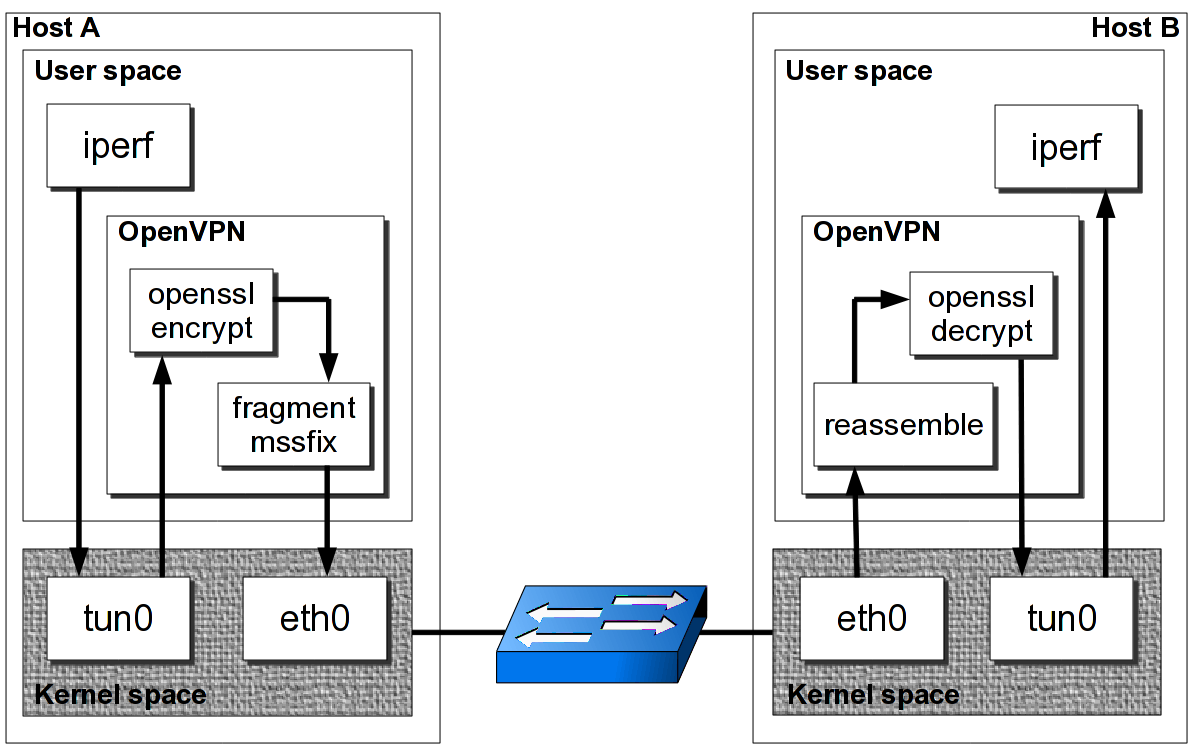
\includegraphics[width=1\textwidth]{./images/packetflow.png}
    \caption{VPN Packets flow}
    \label{packetFlow}
  \end{figure}

  OpenVPN runs in user space which provides good security and portability but packets need to travel between kernel space and user space which is called context switching.
  Context-switching takes CPU cycle, which can impact a lot the performances if the hardware is not powerfull enough.

  On figure \ref{packetFlow} you can see how the packets flow from an application to the network and from the network to the application.

  To create the tunnel OpenVPN uses the tunnel driver that is provided as a module for linux. This driver enable the creation of virtual interfaces called tun or tap devices. The difference between tun and tap are the
  layer at which they are, tap is a layer 2 and tun is a layer 3 device.

  In practice this means that tap is able to send ethernet frame and add more overhead and tun is only able to send packet but add less overhead. For the tests presented in this paper the interface tun is enough and is a better
  choice because it add less overhead.
